\subsection{Spectral Bin Model(SBM)}
The Spectral Bin Model (SBM) was developed by \cite{suzuki_2006} and \cite{suzuki_etal_2010}. The model forecasts the Size Distribution Function (SDF) of seven types of hydrometeors (liquid, plate-ice, columnar-ice, dendritic-ice, snow, graupel, and hail). \\
The SBM calculates mass density of the seven types of hydrometeor and one type of aerosol as their SDFs. The SDF of aerosol can be changed by advection and activation (i.e., nucleation from aerosol to cloud) processes. The SDF of hydrometeors can be changed by several growth processes (i.e., activation from aerosol to cloud, condensation/evaporation, collision/coagulation, freezing/melting, ice nucleation, riming, aggregation, advection, and gravitational falling). \\
The time evolution of SDF (number density) of aerosol ($f_{a}(m,t)$) and SDF (number density) of hydrometeor ($f_{c}(m,t)$) are shown as:

\begin{eqnarray}
\frac{\partial f^{(\mu)}_{c}(m,t)}{\partial t}&=&Adv\bigl[f^{(\mu)}_{c}(m,t)\bigr]+Grav\bigl[f^{(\mu)}_{c}(m,t)\bigr]+\Bigl[ \frac{\partial f^{(\mu)}_{c}(m,t)}{\partial t}\Bigr ]_{cloud\;microphysics}\label{s10-1}\\
\frac{\partial f_{a}(m_{a},t)}{\partial t}&=&Adv\bigl[f_{a}(m_{a},t)\bigr]+Grav\bigl[f_{a}(m_{a},t)\bigr]+\Bigl[ \frac{\partial f_{a}(m_{a},t)}{\partial t} \Bigr ]_{cloud\;microphysics}.\label{s10-2}
\end{eqnarray}

where $\mu$ shows type of hydrometeor (the seven types), and $Adv[]$, $Grav[])$ show change of SDF by  advection and gravitational falling. $\Bigl[ \Bigr]_{cloud\;microphysics}$ shows SDF changes by cloud microphysical processes.\\
The time evolution of $f_{c}^{(\mu)}(m,t)$, and $f_{a}(m,t)$ are shown as:

\begin{eqnarray}
\Bigl[ \frac{\partial f_{c}^{(\mu)}(m,t)}{\partial t}\Bigl]_{cloud\;microphysics}&=&\Bigl[\frac{\partial f_{c}^{(\mu)}(m,t)}{\partial t}\Bigr]_{activation}+\Bigl[\frac{\partial f_{c}^{(\mu)}(m,t)}{\partial t}\Bigr]_{cond/evap}\nonumber\\
&+&\Bigl[\frac{\partial f_{c}^{(\mu)}(m,t)}{\partial t}\Bigr]_{coll/coag/rim/agg}\nonumber\\
&+&\Bigl[\frac{\partial f_{c}^{(\mu)}(m,t)}{\partial t}\Bigr]_{frz}+\Bigl[\frac{\partial f_{c}^{(\mu)}(m,t)}{\partial t}\Bigr]_{melt}\nonumber\\
\Bigl[ \frac{\partial f_{a}(m_{a},t)}{\partial t}\Bigl]_{cloud\;microphysics}&=&\Bigl[\frac{\partial f_{a}(m_{a},t)}{\partial t}\Bigr]_{activation}\nonumber
\end{eqnarray}

where $\Bigl[\;\Bigr]_{***}$ show change of SDF by each cloud growth process. The detail of these processes will be provided later.\\
 The change of SDFs by advection and gravitational falling (i.e., first and second terms of eq.(\ref{s10-1}), and (\ref{s10-2}) ) are calculated by dynamical core of SCALE-RM shown in section 3.


\subsubsection{Discretization of Size Distribution Function(SDF)}
The SDF of aerosol and cloud is predicted as mass density of each particle size ($g_{a}(m_{a})$, $g_{c}^{(\mu)}(m)$). However most equations are given as equations of number density of cloud/aerosol ($f_{c}^{(\mu)}(m,t)$, $f_{a}(m_{a},t)$); the mass density of cloud/aerosol is transferred to the number density of cloud/aerosol ($g_{a}(m_{a},t)=m_{a}g_{a}(m_{a},t)$, $g_{c}^{(\mu)}(m,t)=m^{(\mu)}f_{c}^{(\mu)}(m,t)$).\\
To cover a wide size range (i.e., $2\;\mu m$ $\sim$ $3\;mm$), a logarithmically uniform grid system ($log(m)\equiv \eta$, $log(m_{a})\equiv \eta_{a}$) is used. In this system, the relationship, $\frac{m_{i+1}}{m_{i}}=const.$ is satisfied.

\subsubsection{Activation from aerosol to cloud particles (nucleation process)}
The change of SDFs by activation from aerosol to cloud particles is calculated based on Kohler theory \cite{kohler_1936}. Through this process, aerosols with radii larger than the aerosol critical radius ($r_{a,crit}$) are activated to clouds. The critical radius is given as:

\begin{eqnarray}
r_{a,crit}=\bigl( \frac{4}{27}\frac{A^{3}}{B}\frac{1}{S_{w}}\Bigr )^{1/3}, \:\:\:A=\frac{2\sigma}{R_{v}\rho_{L}T},\:\:\: B=i_{v}\frac{M_{v}}{M_{s}}\frac{\rho_{s}}{\rho_{L}}.\label{s10-3}
\end{eqnarray}

where $S_{w}$, $\sigma$, $R_{v}$, $\rho_{L}$, $T$, $i_{v}$, $M_{v}$, $M_{s}$, and $\rho_{s}$ show supersaturation of water, surface tension of water, vapor gas constant, temperature, van't Hoff factor ($=2$), molecular weight of water, molecular weight of aerosol, and density of aerosol, respectively.\\
At each time step, $r_{a,crit}$ is calculated using temperature, and masses of aerosols with radii > $r_{a,crit}$ are removed from SDF of aerosol and 
transferred to SDF of cloud as newly generated cloud particles.\\
The radii of newly generated clouds correspond to those of aerosols, but if the radii of aerosols are smaller than the lower limit of cloud SDF, the radii of newly generated clouds are set to the smallest size of cloud SDF ($\sim 2 \mu m$).\\
The changes in aerosol and hydrometeor SDF are shown as:

\begin{eqnarray}
\Bigl[\frac{\partial f_{a}}{\partial t}\Bigr]_{activation}&=&-\int_{m_{a,crit}}^{\infty}f_{a}(m_{a},t)dm_{a}\label{s10-4}\\
\Bigl[\frac{\partial f_{c}^{(\mu)}}{\partial t}\Bigr]_{activation}&=&-\Bigl[\frac{\partial f_{a}}{\partial t}\Bigr]_{activation}\label{s10-5}
\end{eqnarray}

where $m_{a,crit}=\bigl(=\frac{4\pi}{3}r_{a}^{3}\rho_{a}$ is mass of aerosol particles with radii the same as critical radii, $r_{a,crit}$. When there is not enough vapor to activate all aerosol particles with radii larger than the critical radius, i.e.,

\begin{eqnarray}
\int_{m_{a,crit}}^{\infty}m_{a}f_{a}(m_{a},t)dm_{a} > q_{v}\rho,\label{s10-6}
\end{eqnarray}

only the aerosol particles with radii > than $r_{a0,crit}$, given as:

\begin{eqnarray}
\int_{m_{a0,crit}}^{\infty}m_{a}f_{a}(m_{a},t)dm_{a} = q_{v}\rho,\label{s10-7}
\end{eqnarray}


are transferred to cloud particles as:

\begin{eqnarray}
\Bigl[\frac{\partial f_{a}}{\partial t}\Bigr]_{activation}&=&-\int_{m_{a0,crit}}^{\infty}f_{a}(m_{a},t)dm_{a},\label{s10-8}\\
\Bigl[\frac{\partial f_{c}^{(\mu)}}{\partial t}\Bigr]_{activation}&=&-\Bigl[\frac{\partial f_{a}}{\partial t}\Bigr]_{activation}.\label{s10-9}
\end{eqnarray}

where $q_{v}$ and $\rho$ is the mixing ratio of water vapor and density.

\subsubsection{Condensation/evaporation}
Calculation of condensation and evaporation processes is based on an equation. The mass change by these two process is given by an equation (e.g., \cite{ry_1989}):

\begin{eqnarray}
\frac{dm}{dt}&=&C^{(\mu)}(m)G^{(\mu)}(T)S^{(\mu)}\\
G^{(\mu)}(T)&=&
\left\{
\begin{array}{l}
G_{w}(T)\;\;\;(\mu : \:liquid)\\
G_{i}(T)\;\;\;(\mu : \:ice)
\end{array}\right. \nonumber\\
G_{w}(T)&=&\frac{4\pi}{\frac{R_{v}T}{e_{w}(T)D_{v}}+\frac{L_{w}}{KT}\bigl( \frac{L_{w}}{R_{v}T}-1\Bigr )}\nonumber\\
G_{i}(T)&=&\frac{4\pi}{\frac{R_{v}T}{e_{i}(T)D_{v}}+\frac{L_{i}}{KT}\bigl( \frac{L_{i}}{R_{v}T}-1\Bigr )}\nonumber\\
S^{(\mu)}&=&
\left\{
\begin{array}{l}
S_{w}\;\;\;(\mu : liquid)\\
S_{i}\;\;\;(\mu : ice)
\end{array}\right.\nonumber
\end{eqnarray}

where $C^{(\mu)}(m)$ is capacitance, which depends on the shape of each type of hydrometeor, $S_{w}$, $S_{i}$ are super saturation of water and ice, $L_{w}$, $L_{i}$ are sensible heat of evaporation, sublimation, $D_{v}$ is diffusion constant of vapor, $K$ is conductivity of air, and $e_{w}$, $e_{i}$ are saturation vapor pressure and saturation ice pressure, respectively. Condensation (evaporation) occur when $S^{(\mu)}$ is positive (negative).\\
To calculate change of SDF by condensation/evaporation, mass flux ($F^{(\mu)}_{cond/evap}$) on each bin is given by using number density ($f_{c}^{(\mu)}$) and $\frac{dm}{dt}$ as:

\begin{eqnarray}
F^{(\mu)}_{cond/evap}=f^{(\mu)}(m)\frac{dm}{dt}=f^{(\mu)}(m)C^{(\mu)}G^{(\mu)}(T)S^{(\mu)}.\label{s10-10}
\end{eqnarray}

Using this equation, time evolution of SDF ($f^{(\mu)}$) is given as

\begin{eqnarray}
\Bigl[\frac{\partial f^{(\mu)}(m,t)}{\partial t}\Bigr]_{cond/evap}&=&-\frac{\partial}{\partial m}F^{(\mu)}_{cond/evap}(m)\nonumber\\
&=&-\frac{\partial}{\partial m}\bigl (f^{(\mu)}(m)C^{(\mu)}\bigr ) G^{(\mu)}(T)S^{(\mu)}.\label{s10-11}
\end{eqnarray}


By using the $\eta(=\log(m))$, eq.(\ref{s10-11}) is transferred to the advection equation:

\begin{eqnarray}
\frac{\partial f^{(\mu)}(\eta)}{\partial t}&=&-\frac{\partial}{\partial \eta}\bigl ( f^{(\mu)}(\eta)U^{(\mu)}(\eta)\bigr)\label{s10-12}\\
U^{(\mu)}(\eta)&=&\frac{C^{(\mu)}(\eta)}{\exp (\eta)}G^{(\eta)}(T)S^{(\eta)}.\nonumber
\end{eqnarray}

To solve eq.(\ref{s10-12}), a scheme developed by \cite{bott_1989} is used. The number density of the i-th bin after $\Delta t$ ($f_{i}(t+\Delta t)$) is given as follows:

\begin{eqnarray}
f_{i}(t+\Delta t)&=&f_{i}(t)-\frac{\Delta t}{\Delta \eta}\bigl [F_{cond/evap,i+1/2}-F_{cond/evap,i-1/2}\Bigr ].\nonumber\\
F_{cond/evap,i+1/2}&=&\frac{\Delta \eta}{\Delta t}\Bigl[ \frac{i^{+}_{l,i+1/2}}{i_{l,j}}f_{i}(t)-\frac{i^{-}_{l,i+1/2}}{i_{l,i+1}}f_{i+1}(t)\Bigr ]\nonumber\\
i^{+}_{l,i+1/2}&=&max\bigl(0,I^{+}_{l}(c_{i+1/2})\bigr)\nonumber\\
i^{-}_{l,i+1/2}&=&max\bigl(0,I^{-}_{l}(c_{i+1/2})\bigr)\nonumber\\
i^{+}_{l,i}&=&max\bigl(I_{l,i},i^{+}_{l,i+1/2}+i^{-}_{l,i+1/2})\bigr)\nonumber\\
I^{+}_{l}(c_{i+1/2})&=&\sum_{k=0}^{2}\frac{a_{i,k}}{(k+1)2^{k+1}}\bigl[1-(1-2c^{+}_{j})^{k+1}\bigr]\nonumber\\
I^{-}_{l}(c_{i+1/2})&=&\sum_{k=0}^{2}\frac{a_{i+1,k}}{(k+1)2^{k+1}}(-1)^{k}\bigl[1-(1-2c^{-}_{j})^{k+1}\bigr]\nonumber\\
a_{i,0}&=&-\frac{1}{24}\bigl( f_{i+1}(t)-26f_{i}(t)+f_{i-1}(t) \bigr)\nonumber\\
a_{i,1}&=&\frac{1}{2}\bigl( f_{i+1}(t)-f_{i-1}(t) \bigr)\nonumber\\
a_{i,2}&=&\frac{1}{2}\bigl( f_{i+1}(t)-2f_{i}(t)+f_{i-1}(t) \bigr)\nonumber\\
c_{i}^{\pm}&=&\pm\bigl( c^{n}_{i+1/2}\pm | c^{n}_{i+1/2}|\bigr )/2\nonumber\\
c^{n}_{i+1/2}&=&U^{n}_{i+1/2}\frac{\Delta t}{\Delta \eta}
\end{eqnarray}

Since super saturation ($S^{(\mu)}$) can change during time step ($\Delta t$), we apply a method shown below to reflect the change of supersaturation during $\Delta t$.\\
Time evolution of supersaturation can be given by equations:

\begin{eqnarray}
\frac{d}{dt}\left(
\begin{array}{l}
S_{w}\\
S_{i}\\
\end{array}\right )
&=&
\left(
\begin{array}{cc}
a_{c/e}& b_{c/e}\\
c_{c/e}& d_{c/e}
\end{array}\right)
\left(
\begin{array}{l}
S_{w}\\
S_{i}
\end{array}\right)
=
A
\left(
\begin{array}{l}
S_{w}\\
S_{i}
\end{array}\right)\label{s10-13}\\
a_{c/e}&=&-(S_{w}+1)\Bigl(\frac{1}{q_{v}}+\frac{L_{w}}{R_{v}T^{2}}\frac{L_{w}}{C_{p}}\Bigr )\int f^{(w)}(m)C^{(w)}(m)dm G_{w}(t)\nonumber\\
b_{c/e}&=&-(S_{w}+1)\Bigl(\frac{1}{q_{v}}+\frac{L_{w}}{R_{v}T^{2}}\frac{L_{i}}{C_{p}}\Bigr ) \sum_{\mu \in ice}\int f^{(\mu)}(m)C^{(\mu)}(m)dm G_{i}(t)\nonumber\\
c_{c/e}&=&-(S_{i}+1)\Bigl(\frac{1}{q_{v}}+\frac{L_{i}}{R_{v}T^{2}}\frac{L_{w}}{C_{p}}\Bigr ) \int f^{(w)}(m)C^{(w)}(m)dm G_{w}(t)\nonumber\\
d_{c/e}&=&-(S_{i}+1)\Bigl(\frac{1}{q_{v}}+\frac{L_{i}}{R_{v}T^{2}}\frac{L_{i}}{C_{p}}\Bigr ) \sum_{\mu \in ice}\int f^{(\mu)}(m)C^{(^mu)}(m)dm G_{i}(t)\nonumber
\end{eqnarray}


where $q_{v}$ is the mixing ratio of vapor. \\
Using eigen value of $A$ ($\Lambda_{+}$, $\Lambda_{-}$ ($\Lambda_{+}>\Lambda_{-})$), and assuming $a_{c/e}$, $b_{c/e}$, $c_{c/e}$, $d_{c/e}$ are constant during $\Delta t$, average value of super saturation ($\bar{S}_{w,i}(t)$) during $\Delta t$ is given as:

\begin{eqnarray}
\bar{S}_{w}(t)=\frac{1}{\Delta t}\int_{t}^{t+\Delta t}S_{w}(\tau)d\tau&=&b\frac{e^{\Lambda_{+}\Delta t}-1}{\Lambda_{+}\Delta t}S_{+}(t)+b\frac{e^{\Lambda_{-}\Delta t}-1}{\Lambda_{-}\Delta t}S_{-}(t)\nonumber\\
\bar{S}_{i}(t)=\frac{1}{\Delta t}\int_{t}^{t+\Delta t}S_{i}(\tau)d\tau&=&(\Lambda_{+}-a)\frac{e^{\Lambda_{+}\Delta t}-1}{\Lambda_{+}\Delta t}S_{+}(t)+(\Lambda_{-}-a)\frac{e^{\Lambda_{-}\Delta t}-1}{\Lambda_{-}\Delta t}S_{-}(t)\nonumber\\
S_{+}(t)&=&\frac{(\Lambda_{-}-a)S_{w}(t)-bS_{i}(t)}{b(\Lambda_{-}-\Lambda_{+})}\nonumber\\
S_{+}(t)&=&\frac{(a-\Lambda_{+})S_{w}(t)+bS_{i}(t)}{b(\Lambda_{-}-\Lambda_{+})}\nonumber
\end{eqnarray}

The averaged super saturation ($\bar{S}_{w,i}(t)$) is used to solve the eq.(\ref{s10-13}).

\subsubsection{Collision/coagulation/riming/aggregation}
Collision/coagulation processes are calculated by solving stochastic collision equations (e.g., \cite{pk_1997}):

\begin{eqnarray}
\frac{\partial f(m)}{\partial t}&=&\int_0^{m/2}f(m')f(m-m')K(m',m-m')dm' \nonumber\\
&-&f(m)\int_0^{\infty}f(m'')K(m,m'')dm''\label{s10-14}
\end{eqnarray}

where $K(m,m')$ is collection kernel function. Three types of kernel function, i.e., Long type kernel (\cite{long_1974}), Golovin type kernel (\cite{Golovin_1963}), and Hydro-dynamic dynamic kernel as shown in eq.(\ref{s10-15}), are implemented into the SCALE-RM.

\begin{eqnarray}
K(m,m')=\pi(r(m)-r(m'))\left| V(m)-V(m')\right |E_{col}(m,m')E_{coag}(m,m')\label{s10-15}
\end{eqnarray}

where $r(m)$ is radius of hydrometeors with mass $m$ and $V(m)$ is terminal velocity of hydrometeors. The terminal velocity of each species of hydrometeor and each size are shown in Figure \ref{figs10-term} $E_{col}$, and $E_{coag}$ are collision efficiency and coagulation efficiency, respectively.\\

\begin{figure}[ht]
\begin{center}
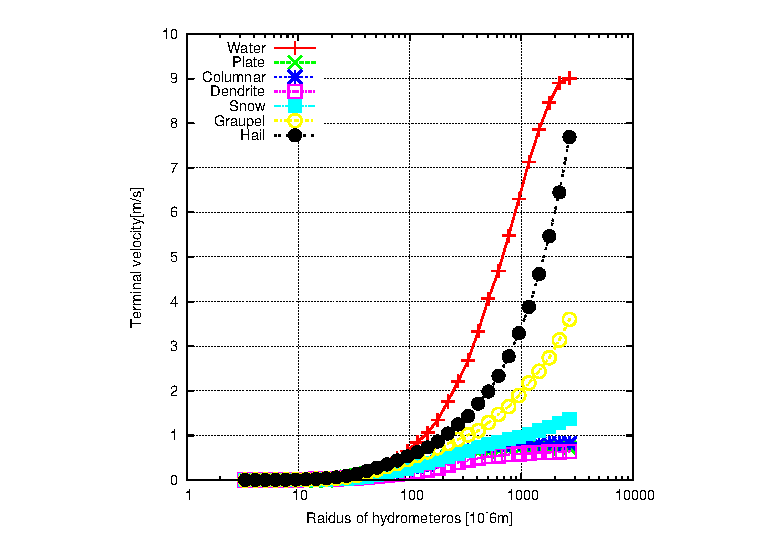
\includegraphics[scale=0.9]{./../figure/terminal-velocity.eps}
\end{center}
\caption{Terminal velocity of Water (Plus), plate-type ice (cross), columnar-type ice (asterisk), dendritic-type ice (open square), snow (closed square), graupel (open circle), and hail (closed circle). Cited from Figure A3 of \cite{suzuki_2006} and rearranged.}
\label{figs10-term}
\end{figure}


Although the stochastic collision equation can be applied for collision/coagulation of one type of hydrometeor (i.e., liquid water), SCALE-RM predicts seven types of hydrometeors and interactions of these types (i.e., riming/aggregation) must be calculated. To calculate the interaction of all seven types of hydrometeors, the extended stochastic collision equation:

\begin{eqnarray}
\Bigr[\frac{\partial f^{(\mu)}(m)}{\partial t}\Bigr]_{coll/coag/rim/agg}&=&\nonumber\\
\sum_{\lambda}\sum_{\nu}\int_{0}^{m/2}f^{(\lambda)}&(&m')f^{(\nu)}(m-m')K_{\lambda\nu}(m',m-m')dm' \nonumber\\
-f^{(\mu)}(m)\sum_{\kappa}\int_0^{\infty}f^{(\kappa)}&(&m'')K_{\kappa\mu}(m,m'')dm''\label{s10-16}
\end{eqnarray}

is applied (where $\mu$, $\nu$, $\lambda$, $\kappa$ represent species of hydrometeor). The combinations of $\mu$, $\nu$, $\lambda$ are shown in table \ref{table-s10-1}.

\begin{table}[h]
\begin{center}
\caption{Catalog of interaction between seven species. W, I, S, G, and H show water, ice, snow, graupel, and hail, respectively. G/H shows graupel(hail) generated when T is lower(higher) than 270.15 K}
\label{table-s10-1}
\begin{tabular}{cccccc}
\hline
     & W   & I   & S   & G   & H   \\ \hline\hline
W    & W   & G/H & G/H & G/H & G/H \\ \hline
I    & I   & S   & S   & I   & I   \\ \hline
S    & S   & S   & S   & S   & S   \\ \hline
G    & G/H & G/H & G   & G   & G/H \\ \hline
H    & G/H & G/H & G/H & G/H & H   \\ \hline
\end{tabular}
\end{center}
\end{table}


To solve the stochastic collision equation, a scheme developed by \cite{bott_1998} was implemented into SCALE-RM.\\
The \cite{bott_1998} scheme calculates evolution of mass density distribution ($g(\eta)=mf(\eta)$, $\eta=\log(m)$). The stochastic collision equation can be transferred to:

\begin{eqnarray}
\frac{\partial g(\eta)}{\partial t}&=&\int_{\eta_{0}}^{\eta_{1}}\frac{m^{2}}{(m-m')^{2} m'}g(\eta-\eta') K(\eta-\eta',\eta')g(\eta')d\eta' \nonumber\\
&-&\int_{\eta_{0}}^{\infty} g(\eta)\frac{K(\eta,\eta')}{m'}g(\eta')d\eta'.\label{s10-17}
\end{eqnarray}

 where $\eta_{1}=\log(m/2)$. Decreases of mass of i-th bin and j-th bin are given by:

\begin{eqnarray}
\frac{\partial g_{i}^{(\mu)}}{\partial t}=-\Delta g^{(\mu)}_{i} K_{\mu\nu}(i,j)\frac{g_{j}^{(\nu)}}{m_{j}}\Delta \eta\label{s10-18}
\end{eqnarray}

and


\begin{eqnarray}
\frac{\partial g_{j}^{(\mu)}}{\partial t}=-\Delta g^{(\nu)}_{j}K_{\mu\nu}(i,j)\frac{g_{i}^{(\mu)}}{m_{i}}\Delta \eta\label{s10-19}
\end{eqnarray}

respectively. The terms corresponds to the second term of the right-hand side of eq.(\ref{s10-17}). Eqs.(\ref{s10-18}) and (\ref{s10-19}) can transfer to:

\begin{eqnarray}
\Delta g_{i}^{(\mu)}=g_{i}^{(\mu)}\Bigl [1-\exp\bigl(-K_{\mu\nu}(i,j)\frac{g^{(\nu)}_{j}}{m_{j}}\Delta \eta\Delta t\bigr) \Bigl]\label{s10-20}\\
\Delta g_{j}^{(\nu)}=g_{j}^{(\nu)}\Bigl [1-\exp\bigl(-K_{\mu\nu}(i,j)\frac{g^{(\mu)}_{i}}{m_{i}}\Delta \eta\Delta t\bigr) \Bigl].\label{s10-21}
\end{eqnarray}

The sum of $\Delta g_{i}^{(\mu)}$ and $\Delta g_{j}^{(\nu)}$ corresponds to newly generated mass by collision of hydrometeors with mass of $m_{i}$ and $m_{j}$. The newly generated mass ($g'=\Delta g_{i}^{(\mu)}+\Delta g_{j}^{(\nu)}$,  corresponds to the first term of the right-hand side of eq.(\ref{s10-17})) added k-th bin ($m_{k}=m_{i}+m_{j}$). Since $m_{k}$ is not always bin center, newly generated mass is divided to the k-th and k+1-th bin, as follows.\\
The production of k-th and k+1-th bin is represented as:

\begin{eqnarray}
\Delta g_{k}^{(\lambda)}&=&g_{k}^{\lambda}+g'-\zeta\label{s10-22}\\
\Delta g_{k+1}^{(\lambda)}&=&g_{k+1}^{\lambda}+\zeta\label{s10-23}\\
\zeta&=&\frac{g'}{g_{k}^{(\lambda)}+g'}\sum_{s=0}^{2}\frac{a_{k,s}}{(s+1)2^{k+1}}[1-(1-2c_{k})^{k+1}]\nonumber\\
c_{k}&=&\frac{m'-m_{k}}{m_{k+1}-m_{k}}\nonumber\\
a_{k,0}&=&-\frac{1}{24}(g_{k+1}^{(\lambda)}-26g_{k}^{(\lambda)}+g_{k-1}^{(\lambda)})\nonumber\\
a_{k,1}&=&-\frac{1}{2}(g_{k+1}^{(\lambda)}-g_{k-1}^{(\lambda)})\nonumber\\
a_{k,2}&=&-\frac{1}{2}(g_{k+1}^{(\lambda)}-2g_{k}^{(\lambda)}+g_{k-1}^{(\lambda)})\nonumber
\end{eqnarray}

This procedure is applied for all bins of all types of hydrometeors.\\
In addition, for more rapid calculation, \cite{sato_etal_2009}’s scheme is also implemented into SCALE-RM.

\subsubsection{Freezing}
The calculation of the freezing process is based on a parameterization by \cite{bigg_1953}. The parameterization calculates number density of water ($f_{c}^{(w)}$) that can be frozen:

\begin{eqnarray}
\frac{\partial}{\partial t}f^{(w)}(m)&=&-\frac{f^{(w)}(m)}{\tau_{fr}}\label{s10-24}\\
\tau_{fr}&=&\frac{\exp \bigl[b_{fr}(T_{0}-T)\bigr]}{a_{fr} m}\nonumber
\end{eqnarray}

where $a_{fr}=10^{-4}s^{-1}$, and $b_{fr}=0.66^{o}C^{-1}$ are empirical parameters, and $T_{0}$ is 273.15 $K$.\\
Eq.(\ref{s10-24}) can transfer to:

\begin{eqnarray}
\frac{\partial g^{(w)(m)}}{\partial t}&=&-\frac{g^{(w)}(m)}{\tau_{fr}(m)}\\
\tau_{fr,i}&=&\frac{\exp\bigl (b_{fr}(T_{0}-T)\bigr )}{a_{fr}m}\nonumber
\end{eqnarray}

From this equation, the mass change of i-th bin during $\Delta t$ is given as:

\begin{eqnarray}
g_{i}^{(w)}(t+\Delta t)=g_{i}^{(w)}-Frz_{i}\\
\left \{
\begin{array}{r}
g_{i}^{(plate)}(t+\Delta t)=g_{i}^{(plate)}+Frz_{i}\:\:\: (r_{w}<200\mu m)\\
g_{i}^{(hail)}(t+\Delta t)=g_{i}^{(hail)}+Frz_{i}\:\:\: (r_{w}>200\mu m)
\end{array} \right.\label{s10-26}\\
Frz_{i}=g_{i}^{(w)}(t)\Bigl [1-\exp\bigl (-\frac{\Delta t}{\tau_{fr,i}}\bigr )\bigr]\nonumber
\end{eqnarray}


 As shown in eq.(\ref{s10-26}), the mass of liquid is transferred to plate type ice ($r_{w}<200\mu m$) or hail ($r_{w}>200\mu m$).

\subsubsection{Melting}
The calculation of the melting process is too simple, with all ice particles (i.e., plate, columnar, dendritic, snow, graupel and hail) melting immediately when the temperature is > $T_{0}=273.15$ $K$. This is too simplistic to represent ice phase processes, and we will modify this method in the near future.


